\section{Modélisation d'un document \xml}
La structure d'un document \xml est modélisée de manière relativement classique. On notera l'utilisation d'un \emph{design pattern} \og composite \fg.
Seule la classe \kw{Node} est abstraite.
\begin{figure}[H]
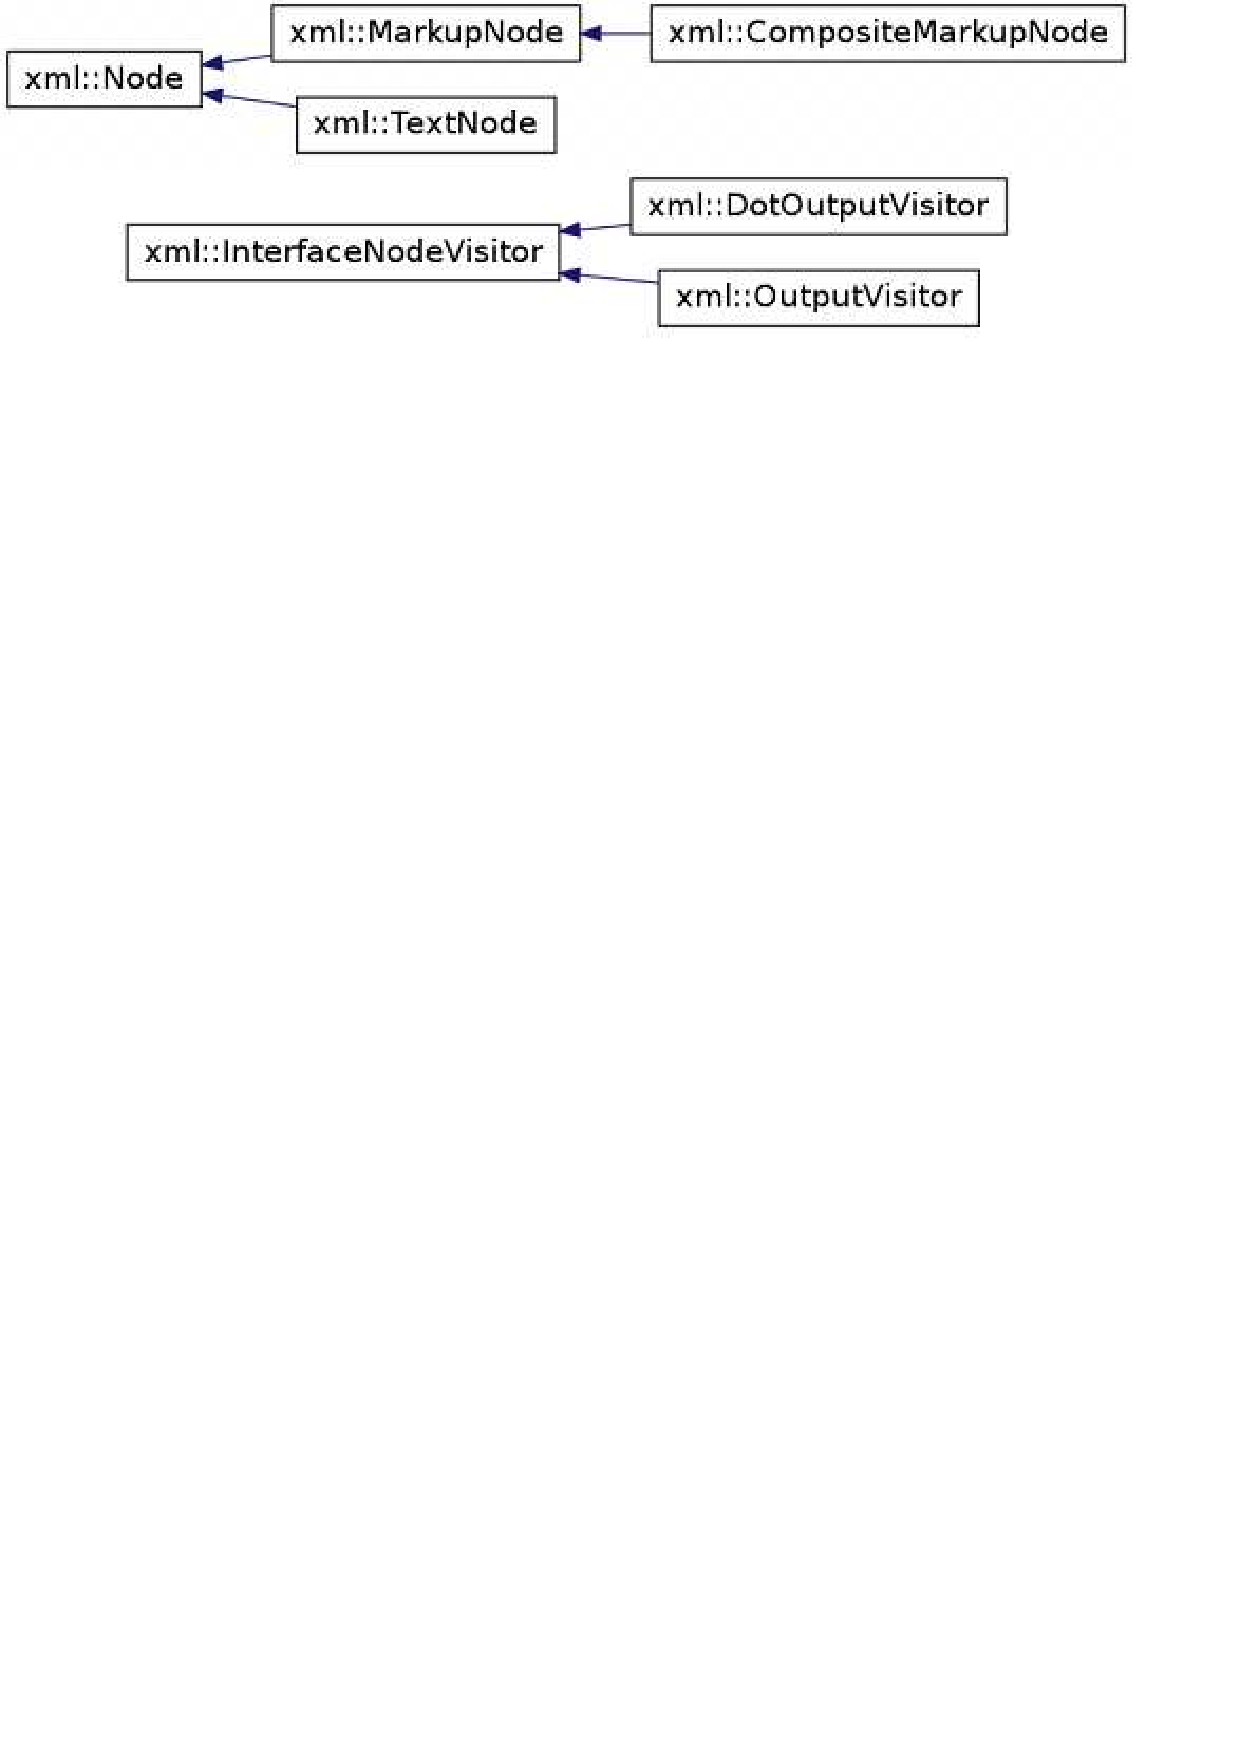
\includegraphics{xml_complet_resume.pdf}
\caption{Diagramme de classes compact du parser XML}
\end{figure}

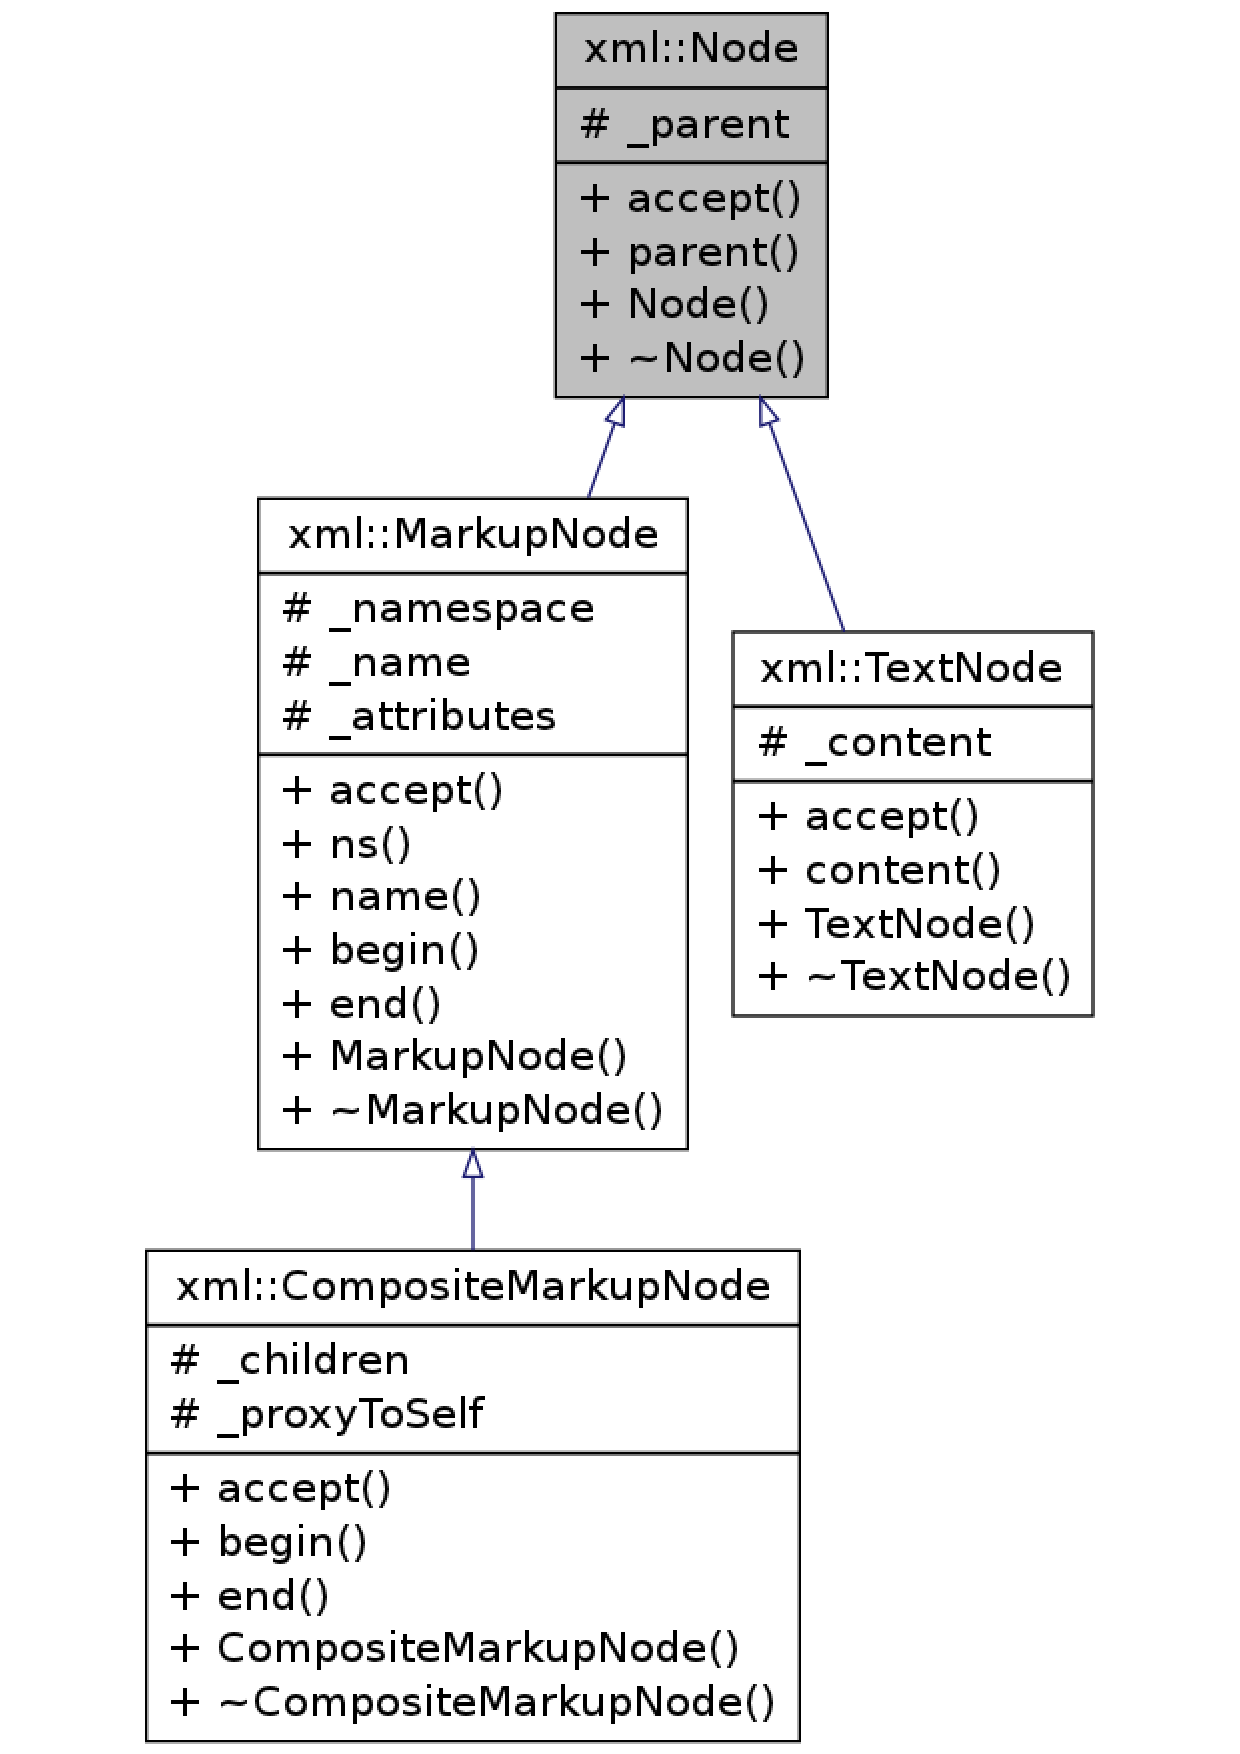
\includegraphics{Xml_node_hierarchie.pdf}
\classDef{Node}
Classe racine abstraite. \\
Elle définit une méthode pour accéder au noeud parent et une méthode abstraite permettant d'accepter un visiteur.
\classDef{MarkupNode}
Classe instanciable représentant une balise vide (de type \kw{<balise />}, sans contenu) dans l'arbre \xml. \\
Elle permet de parcourir ses attributs (au sens \xml) en lecture seule, ainsi que d'accéder à son espace de nom et son nom.
\classDef{CompositeMarkupNode}
Classe instanciable représentant une balise non vide (de type \kw{<balise>...</balise>}, avec éventuellement du contenu) dans l'arbre \xml. \\
Elle permet de parcourir ses noeuds fils en lecture seule, ainsi que toutes les opérations définies par \kw{MarkupNode}.
\classDef{TextNode}
Classe instanciable représentant un texte inclus dans une balise (de type \kw{PCDATA}) dans l'arbre \xml. \\
Elle permet d'accéder à son contenu texte en lecture seule.
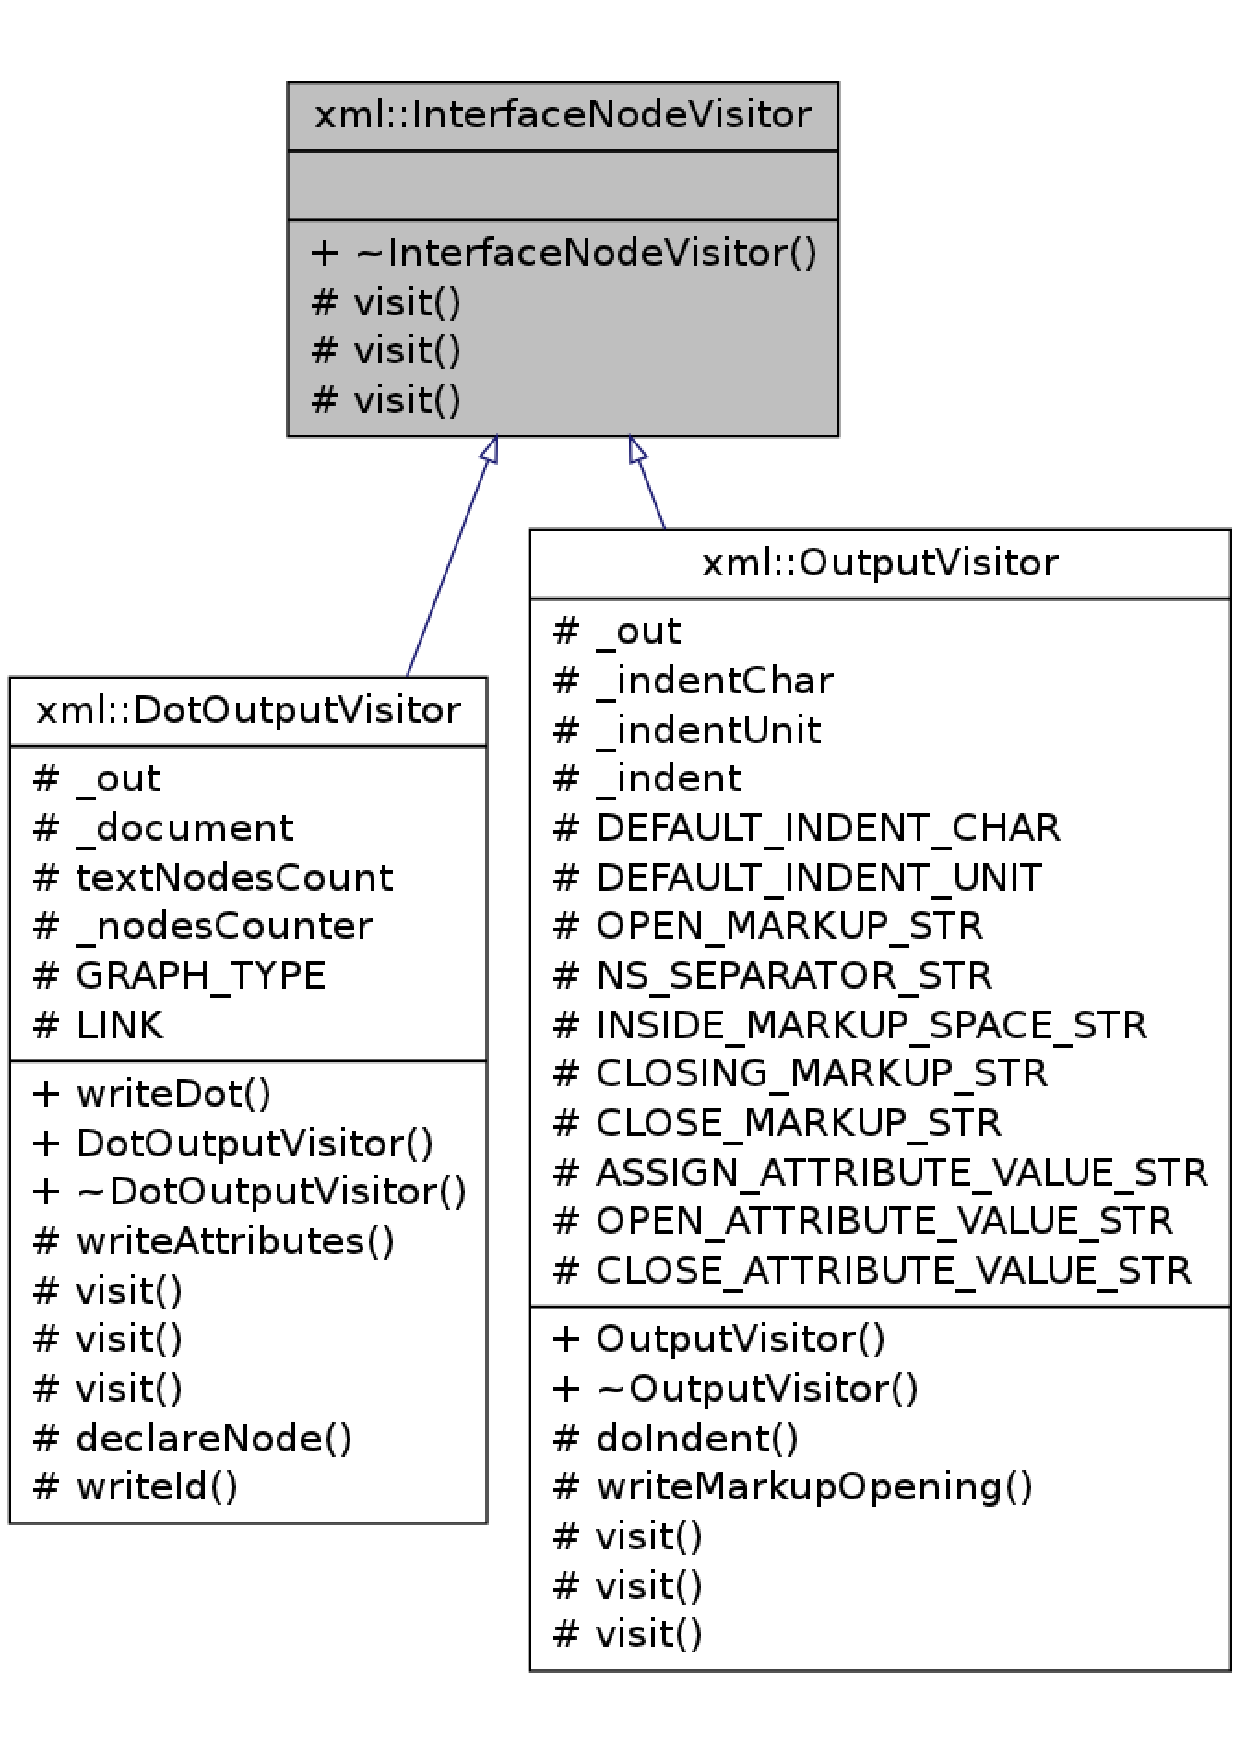
\includegraphics{Xml_visitor.pdf}
